% BORRADOR EN ESPAÑOL para revisión (se traduce al inglés al final).
% Formato final: Behavior Research Methods (APA 7, apa7.cls). Las tablas y figuras se generan
% con simulation/scripts/40_make_tables.R a partir de los CSV de resultados; no se escriben a mano.
% Los decimales llevan punto (no coma) para que el paso a inglés no altere ninguna cifra.
\documentclass[man,donotrepeattitle,floatsintext]{apa7}

\usepackage[T1]{fontenc}
\usepackage[utf8]{inputenc}
\usepackage[spanish,es-nodecimaldot]{babel}
\usepackage{amsmath}
\usepackage{csquotes}
\usepackage[backend=biber,style=apa,sortcites=true,sorting=nyt]{biblatex}
\DeclareLanguageMapping{spanish}{spanish-apa}
\addbibresource{paper_brm.bib}
\graphicspath{{figures/}}
\addto\captionsspanish{\renewcommand{\tablename}{Tabla}\renewcommand{\figurename}{Figura}}

\makeatletter
\newcommand{\blindtext}[2]{\@ifundefined{apaSeven@maskauthoridentity}{#1}{#2}}
\makeatother

\title{¿Cuándo funciona y cuándo no el coeficiente $\xi$ de Chatterjee con datos psicológicos? Una guía basada en simulación y datos reales}
\shorttitle{El coeficiente $\xi$ de Chatterjee en datos psicológicos}

\authorsnames{Arquímedes Chacón}
\authorsaffiliations{Universidad Católica Andrés Bello, Caracas, Venezuela}
\authornote{Correspondencia: Arquímedes Chacón, Universidad Católica Andrés Bello, Caracas, Venezuela. Correo electrónico: arquimedeschacon@gmail.com}

\leftheader{Chacón}

\abstract{El coeficiente $\xi$ de Chatterjee (2021) promete detectar cualquier dependencia funcional entre dos variables mediante una prueba asintótica simple, lo que lo hace atractivo para la psicología, donde son frecuentes las relaciones no monótonas (U invertida, formas en U). Se desconoce, sin embargo, cómo se comporta con los datos típicos de la disciplina: variables binarias u ordinales con empates, tamaños de muestra moderados y efectos débiles. Este artículo lo evalúa en tres estudios reproducibles. El Estudio 1 examina por simulación el error Tipo I y la potencia de su prueba con respuestas binarias, ordinales y puntajes compuestos. El Estudio 2 lo compara con Spearman, Pearson, la correlación de distancia (dCor) y $\tau^*$ en cuatro estructuras de dependencia, calibradas según la varianza explicada y con tamaños de muestra de 50 a 800. El Estudio 3 analiza de forma exhaustiva 645 pares de variables de tres bases públicas (\texttt{bfi}, \texttt{sat.act} y NHANES 2017--2018). La prueba de $\xi$ con ajuste por empates conserva su nivel, salvo con respuestas binarias muy desbalanceadas, donde es anticonservadora; la versión que supone variables continuas falla con respuestas discretas. $\xi$ es, con diferencia, la medida más potente ante relaciones oscilatorias, pero requiere unas ocho veces más participantes que Spearman en relaciones monótonas y, en los datos reales, no detectó ninguna asociación que Spearman y Pearson no detectaran; dCor y $\tau^*$ sí revelaron asociaciones no monótonas, como la forma de U entre sueño y depresión. Además, con ítems tipo Likert el valor de $\xi$ varía con el desempate aleatorio tanto como su propio tamaño. Se ofrece una guía práctica, y todo el código y los resultados son públicos.}

\keywords{coeficiente de Chatterjee, dependencia no monótona, empates, datos ordinales, simulación Monte Carlo, correlación de distancia}

\begin{document}
\maketitle

\section{Introducción}

Muchas teorías psicológicas predicen relaciones que no son monótonas. La ley de Yerkes y Dodson \parencite{yerkes1908} sostiene que el rendimiento mejora con la activación hasta un nivel óptimo y empeora después; la literatura sobre comportamiento organizacional describe el efecto de <<demasiado de algo bueno>>, según el cual rasgos o conductas beneficiosos dejan de serlo en niveles altos \parencite{pierce2013}; y en salud mental tanto dormir poco como dormir mucho se asocian con un mayor riesgo de depresión \parencite{zhai2015}. Sin embargo, los coeficientes que dominan la práctica --la correlación de Pearson y la de Spearman-- miden asociación lineal o monótona y pueden ser cercanos a cero incluso cuando una variable es función exacta de la otra, si esa función no es monótona \parencite{chatterjee2021}. Un investigador que se limite a ellos puede concluir que <<no hay relación>> donde sí la hay.

Existen medidas que detectan dependencias generales. La correlación de distancia (dCor; \cite{szekely2007}) y el coeficiente $\tau^*$ de Bergsma y Dassios \parencite{bergsma2014} valen cero solo bajo independencia, pero sus pruebas son computacionalmente más costosas (permutación, en el caso de dCor). El coeficiente $\xi_n$ de \textcite{chatterjee2021} es una propuesta reciente con ventajas atractivas para quien analiza datos: se calcula con rangos en tiempo $O(n\log n)$, vale cero solo bajo independencia y uno solo si $Y$ es función de $X$, y su distribución bajo independencia es asintóticamente normal, de modo que ofrece una prueba de independencia sin remuestreo. Su aparición ha generado rápidamente una literatura teórica sobre la dependencia condicional \parencite{azadkia2021}, la reducción del sesgo \parencite{dalitz2024}, familias de coeficientes \parencite{gao2024}, umbrales de detección \parencite{auddy2024} y continuidad \parencite{ansari2026,bucher2025}, y existe una implementación estándar en R \parencite{chatterjee2023xicor}.

No obstante, la teoría y las simulaciones publicadas sobre $\xi_n$ se refieren sobre todo a variables continuas, sin empates, y a efectos fuertes. Los datos psicológicos suelen ser otra cosa: ítems de pocas categorías ordenadas, variables binarias, puntajes compuestos, muestras de decenas o cientos de participantes y efectos débiles, en los que una variable explica apenas un pequeño porcentaje de la varianza de la otra. Dos rasgos de $\xi_n$ hacen que los empates importen de manera especial. Primero, cuando hay empates en $X$, su definición exige ordenar al azar las observaciones empatadas, de modo que el valor calculado es una variable aleatoria: dos analistas con los mismos datos pueden obtener valores distintos. Segundo, cuando $Y$ tiene empates, la varianza asintótica del estadístico bajo independencia depende de la distribución de $Y$ \parencite{chatterjee2021}, de modo que una prueba que suponga $Y$ continua puede no tener el nivel nominal. A ello se suman prácticas habituales como dicotomizar variables continuas \parencite{maccallum2002} o tratar escalas ordinales como si fueran continuas \parencite{liddell2018}.

Hasta donde se ha podido establecer, no existe una evaluación sistemática del error Tipo I y de la potencia de $\xi_n$ con este tipo de datos, ni una comparación con las alternativas en una escala de intensidad de la dependencia que no favorezca a ninguna medida, ni una aplicación exhaustiva a bases de datos psicológicas reales. Sin esa evidencia, quien investiga no sabe cuándo puede confiar en $\xi_n$, cuándo es preferible otra medida ni cómo debe reportarlo.

Este trabajo aporta esa evidencia mediante tres estudios, todos con código y resultados públicos y reproducibles. El Estudio 1 evalúa por simulación el nivel y la potencia de la prueba de $\xi_n$ cuando $X$ e $Y$ son binarias, ordinales o puntajes compuestos, con tamaños de muestra de 50 a 1000. El Estudio 2 compara $\xi_n$ con Spearman, Pearson, dCor y $\tau^*$ en cuatro estructuras de dependencia, calibradas según la proporción de varianza explicada por la estructura y no según la escala de ningún coeficiente. El Estudio 3 aplica las cinco medidas a todos los pares de variables de tres bases públicas (645 pares), con una regla de análisis fijada de antemano. El artículo concluye con una guía práctica sobre cuándo usar $\xi_n$, cuándo preferir otra medida y cómo reportarlo.

\section{El coeficiente $\xi_n$ y sus competidoras}

\subsection{Definición y propiedades}

Sean $(X_i,Y_i)$, $i=1,\dots,n$, pares independientes. Se ordenan los pares de modo que $X_{(1)}\le\dots\le X_{(n)}$ (los empates en $X$ se resuelven al azar), se llama $r_i$ al rango de $Y_{(i)}$ entre todos los $Y_j$ y $l_i$ al número de $j$ tales que $Y_j\ge Y_{(i)}$. El coeficiente es
\begin{equation}
\xi_n(X,Y) = 1 - \frac{n\sum_{i=1}^{n-1}|r_{i+1}-r_i|}{2\sum_{i=1}^{n} l_i\,(n-l_i)}.
\end{equation}
Converge casi seguramente a un parámetro poblacional $\xi(X,Y)\in[0,1]$ que vale cero si y solo si $X$ e $Y$ son independientes y uno si y solo si $Y$ es función medible de $X$ \parencite{chatterjee2021}. Bajo independencia y con $Y$ continua, $\sqrt{n}\,\xi_n$ converge a una normal de media cero y varianza $2/5$, lo que da una prueba asintótica de independencia que rechaza para valores grandes de $\xi_n$.

Dos propiedades importan para lo que sigue. Primero, $\xi_n$ es direccional: $\xi_n(X,Y)\neq\xi_n(Y,X)$ en general, porque mide en qué grado $Y$ es función de $X$ y no al revés. Segundo, su comportamiento en muestras finitas tiene límites conocidos: con $Y$ continua el máximo posible es $(n-2)/(n+1)$, de modo que con $n$ pequeño no puede aproximarse a uno \parencite{dalitz2024}; el bootstrap no funciona para este estadístico \parencite{dalitz2024} y, en general, no existen intervalos de confianza de nivel exacto que sean significativos \parencite{bucher2025}. Por ello este trabajo reporta pruebas de hipótesis para $\xi_n$, pero no intervalos de confianza.

\subsection{Empates, discretización y puntajes compuestos}

Con variables discretas, la definición de $\xi_n$ obliga a dos decisiones. Los empates en $X$ se resuelven ordenando al azar las observaciones empatadas, de modo que $\xi_n$ es un estadístico aleatorizado y su valor cambia con cada desempate. Los empates en $Y$ cambian los rangos $r_i$ y los conteos $l_i$ y, con ello, la varianza asintótica bajo independencia, que ya no es $2/5$ sino que depende de la ley de $Y$ \parencite{chatterjee2021}. La implementación estándar \parencite{chatterjee2023xicor} estima esa varianza a partir de los datos por defecto (argumento \texttt{ties = TRUE}), mientras que con \texttt{ties = FALSE} usa la fórmula válida para $Y$ continua. En este trabajo se llama <<prueba con ajuste por empates>> a la primera y <<prueba ingenua>> a la segunda. Un puntaje compuesto --el promedio de varios ítems-- toma muchos más valores distintos que un ítem aislado y, por tanto, tiene menos empates; en cambio, dicotomizar una variable continua \parencite{maccallum2002} introduce el máximo de empates posible.

\subsection{Medidas competidoras y cómo compararlas}

Se compara $\xi_n$ con las medidas de la Tabla~\ref{tab:medidas}. No estiman el mismo parámetro poblacional ni comparten escala, de modo que sus magnitudes no son comparables entre sí; se comparan, en cambio, por el nivel y la potencia de sus pruebas, que son probabilidades de rechazo en las mismas condiciones generadoras. Esto exige, además, un criterio de intensidad de la dependencia que no favorezca a ninguna medida: el Estudio 2 lo fija mediante la proporción de varianza de $Y$ atribuible a la estructura determinista (el $R^2$ de la función verdadera), y no mediante el valor de ningún coeficiente.

\begin{table}
\caption{Medidas de asociación comparadas}
\label{tab:medidas}
\begin{threeparttable}
\small
\begin{tabular}{llll}
\toprule
Medida & Qué detecta & Simétrica & Prueba empleada \\
\midrule
Pearson $r$ & Asociación lineal & Sí & $t$ sobre $r$ \\
Spearman $\rho$ & Asociación monótona & Sí & $t$ sobre $\rho$ \\
dCor & Cualquier dependencia & Sí & Permutación \\
$\tau^*$ & Cualquier dependencia & Sí & Asintótica (modo automático) \\
$\xi_n$ & Dependencia funcional de $Y$ sobre $X$ & No & Asintótica con ajuste por empates \\
\bottomrule
\end{tabular}
\begin{tablenotes}[flushleft]
\small
\item \textit{Nota.} dCor: correlación de distancia \parencite{szekely2007}; $\tau^*$: coeficiente de Bergsma y Dassios \parencite{bergsma2014}; $\xi_n$: coeficiente de Chatterjee \parencite{chatterjee2021}. Las pruebas se describen en el método de cada estudio.
\end{tablenotes}
\end{threeparttable}
\end{table}

\section{Estudio 1: nivel y potencia de la prueba de $\xi_n$ con datos discretos}

\subsection{Método}

\paragraph{Datos.} Se generaron variables latentes continuas y las variables observadas se obtuvieron cortando la latente en puntos de corte poblacionales, de modo que el número de casos por categoría varía al azar de una muestra a otra, como en datos reales. $X$ fue continua, binaria 50/50 u ordinal de 5 categorías asimétrica (proporciones .05, .10, .15, .30 y .40). $Y$ fue continua; binaria con proporciones 50/50, 80/20, 90/10 o 95/5; ordinal de 5 categorías asimétrica; ordinal de 7 categorías con efecto suelo (.35, .25, .15, .10, .07, .05 y .03); o un puntaje compuesto de 5 ítems de seis categorías. Cada ítem se obtuvo cortando en sextiles $\theta+\varepsilon_j$, con $\theta$ el rasgo latente estandarizado y $\varepsilon_j\sim N(0,1)$, y el puntaje es el promedio de los cinco ítems.

\paragraph{Nivel (error Tipo I).} Las latentes de $X$ e $Y$ fueron normales estándar independientes. Se combinaron 3 tipos de $X$, 8 de $Y$ y $n\in\{50,100,250,500,1000\}$ (120 celdas, 5000 réplicas cada una; error estándar de Monte Carlo $\approx .003$ con $\alpha=.05$). En cada réplica se calcularon la prueba asintótica con ajuste por empates (\texttt{XICOR} 0.4.1; \cite{chatterjee2023xicor}) y la prueba ingenua, con $\alpha=.05$ y $\alpha=.01$. Como criterio se usó la banda liberal de robustez de \textcite{bradley1978}: tasas de rechazo entre .025 y .075 con $\alpha=.05$. En 24 celdas ($X$ continua o binaria; $Y$ continua, binaria 90/10, binaria 95/5 u ordinal de 7 categorías; $n=100,250,500$; 1000 réplicas) se evaluó también una prueba de permutación ($B=499$; $p=(1+\#\{\xi_n^*\ge\xi_n\})/(B+1)$, permutando $Y$ y resolviendo de nuevo los empates de $X$).

\paragraph{Potencia.} $Y=f(X)+\sigma\varepsilon$ con $f(x)=x$ (lineal), $x^2$ (cuadrática) o $\sin(2\pi x)$ (sinusoidal), y $X$ y $\varepsilon$ normales estándar. El nivel de ruido $\sigma$ se calibró en la variable latente continua, antes de discretizar, para que $\xi=.15$ en cada estructura. Se combinaron 3 estructuras, 3 tipos de $X$, 8 de $Y$ y 5 tamaños de muestra (360 celdas, 2000 réplicas cada una).

\paragraph{Ruido por desempate.} Para cuantificar la variabilidad debida al desempate aleatorio se usaron simulaciones previas del proyecto (\texttt{scripts/03\_h2b.R}, \texttt{05\_h2d.R} y \texttt{06\_h2d\_kvarying.R}), con $n=100$, $\xi\approx .49$ y relación lineal: 300 conjuntos de datos con 20 desempates cada uno para $X$ discretizada, y 1000 réplicas para el puntaje compuesto de 10 ítems (500 en la serie según el número de ítems).

\subsection{Resultados}

\paragraph{Nivel.} La Tabla~\ref{tab:s1nivel} resume el error Tipo I. En 119 de las 120 celdas la prueba con ajuste por empates estuvo dentro de la banda de Bradley (rango .043--.076; la única excepción fue $X$ continua, $Y$ 90/10 y $n=50$, con .076). Con respuestas continuas, ordinales y puntajes compuestos el nivel fue adecuado en todos los tamaños de muestra. Con respuestas binarias muy desbalanceadas la prueba es anticonservadora y la inflación no desaparece al aumentar $n$: con 5 \% en la categoría minoritaria las tasas fueron de .052 a .072 y todavía de .069 con $n=1000$ (unos 50 casos en la categoría minoritaria). En la cola la inflación es mayor: con $\alpha=.01$ las tasas fueron .018 (90/10) y .025 (95/5), cerca del doble y de dos veces y media el nivel nominal. Los resultados no dependieron de que $X$ estuviera discretizada (las tasas promedio por tipo de $Y$ difirieron en menos de .005 entre tipos de $X$).

La prueba ingenua, que supone $Y$ continua, rechazó demasiado con respuestas discretas: tasas promedio de .142 a .154 con respuestas binarias (alrededor del triple del nivel nominal), .084 con la ordinal de 5 categorías y .073 con la de 7. Solo fue adecuada con $Y$ continua y con el puntaje compuesto (.053 y .051), que tiene muchos valores distintos.

\begin{table}
\caption{Error Tipo I de la prueba de $\xi_n$ bajo independencia, con $X$ continua}
\label{tab:s1nivel}
\begin{threeparttable}
\small
\begin{tabular}{lccccccc}
\toprule
 & \multicolumn{5}{c}{Prueba con ajuste por empates, $\alpha = .05$} & Ingenua & Con ajuste \\
\cmidrule(lr){2-6}
Respuesta $Y$ & $n=50$ & $n=100$ & $n=250$ & $n=500$ & $n=1000$ & $\alpha = .05$ & $\alpha = .01$ \\
\midrule
Continua & .051 & .053 & .052 & .058 & .050 & .053 & .010 \\
Binaria 50/50 & .057 & .058 & .048 & .049 & .047 & .152 & .010 \\
Binaria 80/20 & .059 & .055 & .049 & .050 & .051 & .146 & .012 \\
Binaria 90/10 & .076 & .060 & .050 & .050 & .061 & .154 & .018 \\
Binaria 95/5 & .052 & .064 & .072 & .070 & .069 & .142 & .025 \\
Ordinal, 5 cat. (asim\'etrica) & .050 & .056 & .052 & .049 & .050 & .084 & .012 \\
Ordinal, 7 cat. (efecto suelo) & .045 & .047 & .050 & .054 & .049 & .073 & .009 \\
Compuesto de 5 \'items & .052 & .047 & .052 & .048 & .051 & .051 & .009 \\
\bottomrule
\end{tabular}

\begin{tablenotes}[flushleft]
\small
\item \textit{Nota.} Tasas de rechazo (5000 réplicas por celda). La prueba con ajuste por empates es la de \texttt{XICOR} con \texttt{ties = TRUE}; la ingenua usa la varianza válida para $Y$ continua. Las dos últimas columnas promedian los cinco tamaños de muestra. Con $X$ binaria u ordinal los resultados fueron equivalentes (diferencias menores a .005).
\end{tablenotes}
\end{threeparttable}
\end{table}

\paragraph{Remedio: prueba de permutación.} En las 24 celdas evaluadas, la prueba de permutación mantuvo el nivel pero fue conservadora con respuestas binarias desbalanceadas (tasas de .021 a .038 con $\alpha=.05$ y de .010 o menos con $\alpha=.01$), y se comportó como la prueba asintótica con respuestas continuas y ordinales (.037--.062 y .042--.056, respectivamente). Es, por tanto, una alternativa segura, a costa de potencia, cuando la categoría minoritaria es muy pequeña.

\paragraph{Potencia con respuestas discretas.} La discretización de $Y$ reduce la potencia (Figura~\ref{fig:s1}). Con relación lineal y $n=100$ la potencia con $Y$ continua fue .725; con binaria 50/50, .474; con binaria 90/10, .309; con ordinal de 5 categorías, .625; y con el puntaje compuesto, .561. Con $n=250$ las cifras fueron .962, .812, .488, .921 y .888. La pérdida es muy grande con respuestas binarias desbalanceadas y moderada con ordinales y compuestos, y se reduce a menos de .08 desde $n=250$. La excepción es la estructura cuadrática, en la que una respuesta 90/10 detectó mejor que la continua con $n=100$ (.757 frente a .697), posiblemente porque la categoría minoritaria concentra los valores extremos, donde se manifiesta la curvatura.

\begin{figure}
\caption{Potencia de la prueba de $\xi_n$ según el tipo de respuesta}
\label{fig:s1}
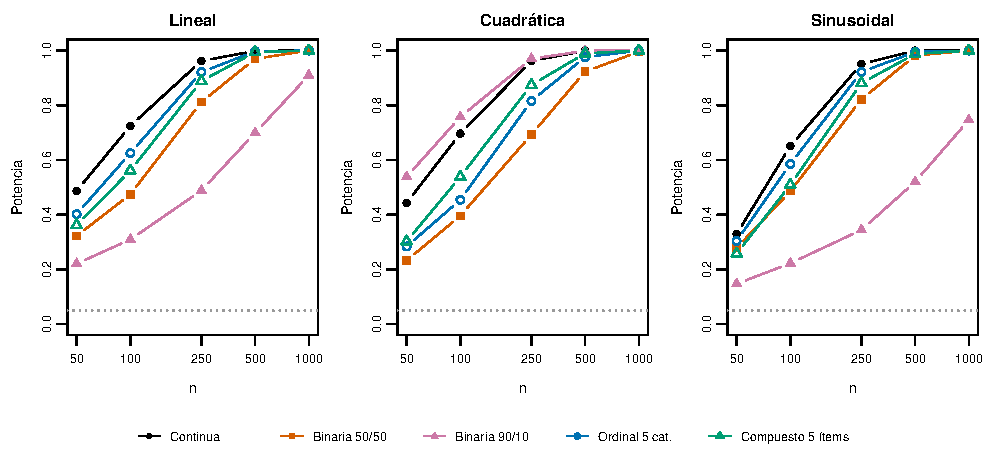
\includegraphics[width=\textwidth]{fig1_study1_es.pdf}
\figurenote{Potencia (2000 réplicas) con $X$ continua y dependencia calibrada a $\xi=.15$ en la variable latente. La línea punteada marca el nivel nominal .05.}
\end{figure}

\paragraph{Discretizar el predictor.} Dicotomizar $X$ elimina la capacidad de $\xi_n$ de detectar relaciones no monótonas (Tabla~\ref{tab:s1x}). Con $n=250$ la potencia con $X$ continua fue .962 (cuadrática) y .951 (sinusoidal); con $X$ binaria 50/50 fue .052 y .056, es decir, el nivel nominal; con $X$ ordinal de 5 categorías, .602 y .182. Con la estructura lineal, dicotomizar $X$ redujo la potencia de .962 a .751.

\begin{table}
\caption{Potencia de $\xi_n$ según la discretización de $X$ ($Y$ continua)}
\label{tab:s1x}
\begin{threeparttable}
\small
\begin{tabular}{lcccccc}
\toprule
 & \multicolumn{3}{c}{$n = 100$} & \multicolumn{3}{c}{$n = 250$} \\
\cmidrule(lr){2-4}\cmidrule(lr){5-7}
Estructura & Continua & Binaria 50/50 & Ordinal, 5 cat. & Continua & Binaria 50/50 & Ordinal, 5 cat. \\
\midrule
Lineal & .725 & .431 & .591 & .962 & .751 & .917 \\
Cuadr\'atica & .697 & .055 & .324 & .962 & .052 & .602 \\
Sinusoidal & .651 & .062 & .110 & .951 & .056 & .182 \\
\bottomrule
\end{tabular}

\begin{tablenotes}[flushleft]
\small
\item \textit{Nota.} Tasas de rechazo con $\alpha=.05$ (2000 réplicas); dependencia calibrada a $\xi=.15$ en la variable latente.
\end{tablenotes}
\end{threeparttable}
\end{table}

\paragraph{Ruido por desempate.} Cuando $X$ está discretizada, parte de la variabilidad de $\xi_n$ no proviene de la muestra sino del desempate aleatorio (Tabla~\ref{tab:s1tb}). Con $X$ binaria, el 44 \% de la variabilidad total se debió solo al desempate, y la proporción disminuyó con más categorías (37 \%, 31 \% y 27 \% con 3, 5 y 7 categorías). Un puntaje compuesto de 10 ítems redujo la varianza empírica de $\xi_n$ un 37 \% respecto de un ítem único (de .0055 a .0035); la mejora se estabilizó desde unos 5 ítems (.0036) y fue muy pequeña con hasta 400 ítems (.0029).

\begin{table}
\caption{Variabilidad de $\xi_n$ entre conjuntos de datos y por desempate aleatorio ($n=100$)}
\label{tab:s1tb}
\begin{threeparttable}
\small
\begin{tabular}{lccc}
\toprule
$X$ discretizada en & Entre conjuntos de datos & Por desempate & \% por desempate \\
\midrule
Continua & .0034 & .0000 & 0 \\
Binaria & .0021 & .0017 & 44 \\
Likert-3 & .0022 & .0013 & 37 \\
Likert-5 & .0024 & .0011 & 31 \\
Likert-7 & .0026 & .0009 & 27 \\
\bottomrule
\end{tabular}

\begin{tablenotes}[flushleft]
\small
\item \textit{Nota.} Varianzas de $\xi_n$ (relación lineal, $\xi\approx .49$; 300 conjuntos de datos con 20 desempates cada uno). La última columna es la parte de la varianza total debida al desempate.
\end{tablenotes}
\end{threeparttable}
\end{table}

\section{Estudio 2: $\xi_n$ frente a medidas competidoras}

\subsection{Método}

\paragraph{Estructuras y calibración neutral.} Se usaron las estructuras lineal, cuadrática y sinusoidal del Estudio 1 y una estructura circular: $X=2\Phi(Z)-1$, uniforme en $(-1,1)$ con $Z$ normal estándar, e $Y=S\sqrt{1-X^2}+\sigma\varepsilon$, con $S=\pm1$ con igual probabilidad, de modo que $Y$ no es función de $X$. La intensidad de la dependencia se fijó con la proporción de varianza de la $Y$ latente atribuible a la estructura determinista, $R^2=\operatorname{Var}(f)/(\operatorname{Var}(f)+\sigma^2)$, es decir, el $R^2$ de la función verdadera, con $\operatorname{Var}(f)$ calculada en una muestra grande sin ruido. Una misma cantidad $R^2$ significa la misma cantidad de señal en las cuatro estructuras, sin referencia al valor de ningún coeficiente. Los valores fueron .05, .13, .26 y .50 (.13 y .26 corresponden a los efectos mediano y grande de Cohen, 1988) y, solo para la estructura circular, .70, .85 y .95, porque con $R^2\le .50$ ninguna prueba tuvo potencia apreciable en esa estructura.

\paragraph{Respuestas y pruebas.} $X$ fue continua. $Y$ fue continua, binaria 50/50, binaria 90/10, ordinal de 5 categorías asimétrica o puntaje compuesto de 5 ítems (definidos como en el Estudio 1). Se compararon (Tabla~\ref{tab:medidas}) la prueba de $\xi_n$ con ajuste por empates; las pruebas $t$ de Spearman y de Pearson; dCor con prueba de permutación ($B=199$; \texttt{energy} 1.7.12, \cite{rizzo2024energy}); y $\tau^*$ con la prueba de \texttt{TauStar} 1.1.9 \parencite{weihs2026taustar}, que elige automáticamente el modo continuo, mixto o discreto según los datos. Todas las pruebas se aplicaron a los mismos conjuntos de datos simulados.

\paragraph{Diseño.} Error Tipo I: $n\in\{50,100,200,400\}$, 5 tipos de $Y$, 1000 réplicas. Potencia, con $\xi_n$, Spearman y Pearson: 4 estructuras, 4 valores de $R^2$, $n\in\{50,100,200,400,800\}$ y 5 tipos de $Y$, con 2000 réplicas. Potencia, con las cinco medidas: $R^2\in\{.13,.26\}$ (y .70, .85 y .95 en la estructura circular), $n\in\{50,100,200,400\}$ y $Y$ continua, binaria 50/50, ordinal o compuesta, con 500 réplicas (error estándar $\le .022$). El tamaño de muestra necesario para una potencia de .80 se interpoló de forma log-lineal entre los tamaños evaluados. Dado que dCor y $\tau^*$ son costosos, solo se evaluaron hasta $n=400$.

\subsection{Resultados}

\paragraph{Nivel.} Las cinco pruebas mantuvieron el nivel (Tabla~\ref{tab:s2nivel}; .039 a .063 con $\alpha=.05$, promediando sobre $n$), salvo $\xi_n$ con $Y$ 90/10, que rechazó .063 con $\alpha=.05$ y .018 con $\alpha=.01$, en consonancia con el Estudio 1. Spearman, Pearson, dCor y $\tau^*$ no mostraron ese problema (.052 a .057 con $Y$ 90/10). La rutina de $\tau^*$ emitió avisos numéricos en el 24 \% de las réplicas con $Y$ 90/10 (hasta alrededor del 32 \% en algunas celdas) y en el 5 \% con $Y$ binaria 50/50, sin que su nivel se alterara.

\begin{table}
\caption{Error Tipo I de las cinco pruebas bajo independencia (promedio sobre $n=50$--$400$)}
\label{tab:s2nivel}
\begin{threeparttable}
\small
\begin{tabular}{lcccccc}
\toprule
Respuesta $Y$ & $\xi_n$ & Spearman & Pearson & dCor & $\tau^*$ & Avisos de $\tau^*$ \\
\midrule
\multicolumn{7}{l}{\emph{Nivel de significaci\'on .05}} \\
Continua & .043 & .049 & .048 & .045 & .049 & 0\% \\
Binaria 50/50 & .046 & .050 & .050 & .042 & .054 & 5\% \\
Binaria 90/10 & .063 & .057 & .057 & .052 & .055 & 24\% \\
Ordinal, 5 cat. (asim\'etrica) & .053 & .043 & .048 & .039 & .044 & 1\% \\
Compuesto de 5 \'items & .049 & .053 & .051 & .049 & .053 & 0\% \\
\midrule
\multicolumn{7}{l}{\emph{Nivel de significaci\'on .01}} \\
Continua & .008 & .012 & .011 & .005 & .010 &  \\
Binaria 50/50 & .009 & .011 & .011 & .006 & .012 &  \\
Binaria 90/10 & .018 & .008 & .013 & .006 & .007 &  \\
Ordinal, 5 cat. (asim\'etrica) & .009 & .008 & .006 & .004 & .007 &  \\
Compuesto de 5 \'items & .009 & .010 & .009 & .005 & .011 &  \\
\bottomrule
\end{tabular}

\begin{tablenotes}[flushleft]
\small
\item \textit{Nota.} Tasas de rechazo (1000 réplicas por celda y tamaño de muestra, $X$ continua). La última columna es la proporción de réplicas en que la rutina de $\tau^*$ emitió un aviso numérico.
\end{tablenotes}
\end{threeparttable}
\end{table}

\paragraph{Potencia.} La Figura~\ref{fig:s2} y la Tabla~\ref{tab:s2n80} muestran que ninguna medida domina. En la relación \emph{lineal}, Pearson y Spearman son las más potentes y $\xi_n$ es mucho menos potente: con $R^2=.13$ e $Y$ continua se necesitan 61 (Pearson) y 68 (Spearman) participantes para una potencia de .80, 74 y 75 con dCor y $\tau^*$, y 527 con $\xi_n$, unas ocho veces más. En la relación \emph{cuadrática}, Pearson y Spearman no detectan nada (potencias de .03 a .17 en las celdas evaluadas; $n_{80}>800$); la medida más potente es dCor ($n_{80}=207$ con $R^2=.13$ y 98 con $R^2=.26$), seguida de $\tau^*$ (314 y 156) y de $\xi_n$ (685 y 206). En la relación \emph{sinusoidal}, solo $\xi_n$ alcanza una potencia de .80 ($n_{80}=484$ con $R^2=.13$ y 136 con $R^2=.26$); con $R^2=.26$ y $n=400$ la potencia de dCor y de $\tau^*$ fue de solo .29 y .30, frente a .998 de $\xi_n$, y Spearman y Pearson no superaron el nivel nominal. Con respuestas ordinales los tamaños de muestra necesarios aumentan (por ejemplo, 647 frente a 527 para $\xi_n$ con $R^2=.13$ en la relación lineal), pero el orden de las medidas no cambia.

\begin{figure}
\caption{Potencia de las cinco medidas según la estructura de dependencia y el tamaño de muestra}
\label{fig:s2}
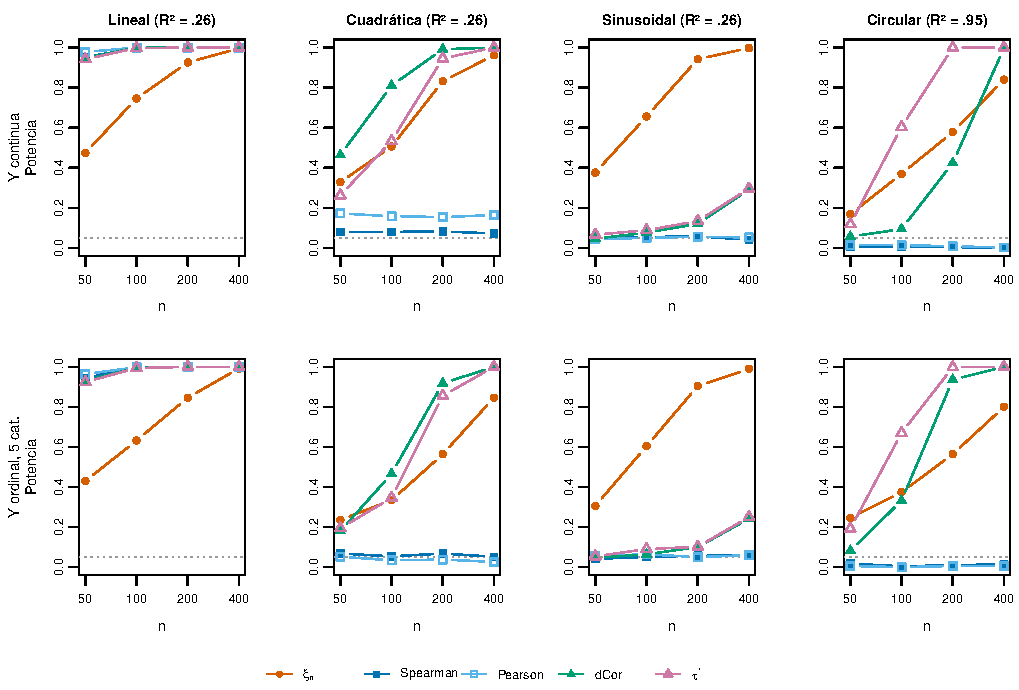
\includegraphics[width=\textwidth]{fig2_study2_es.pdf}
\figurenote{Potencia con $\alpha=.05$ (500 réplicas). $R^2=.26$ en las tres primeras estructuras y $R^2=.95$ en la circular. La línea punteada marca el nivel nominal.}
\end{figure}

\begin{table}
\caption{Tamaño de muestra necesario para una potencia de .80}
\label{tab:s2n80}
\begin{threeparttable}
\small
\setlength{\tabcolsep}{4pt}
\begin{tabular}{lllccccc}
\toprule
Estructura & $R^2$ & Respuesta $Y$ & $\xi_n$ & Spearman & Pearson & dCor & $\tau^*$ \\
\midrule
Lineal & .13 & Continua & 527 & 68 & 61 & 74 & 75 \\
 & .13 & Ordinal, 5 cat. (asim\'etrica) & 647 & 75 & 72 & 81 & 82 \\
 & .26 & Continua & 131 & $<$50 & $<$50 & $<$50 & $<$50 \\
 & .26 & Ordinal, 5 cat. (asim\'etrica) & 162 & $<$50 & $<$50 & $<$50 & $<$50 \\
\addlinespace
Cuadr\'atica & .13 & Continua & 685 & $>$800 & $>$800 & 207 & 314 \\
 & .13 & Ordinal, 5 cat. (asim\'etrica) & $>$800 & $>$800 & $>$800 & 320 & 374 \\
 & .26 & Continua & 206 & $>$800 & $>$800 & 98 & 156 \\
 & .26 & Ordinal, 5 cat. (asim\'etrica) & 378 & $>$800 & $>$800 & 167 & 185 \\
\addlinespace
Sinusoidal & .13 & Continua & 484 & $>$800 & $>$800 & $>$400 & $>$400 \\
 & .13 & Ordinal, 5 cat. (asim\'etrica) & 606 & $>$800 & $>$800 & $>$400 & $>$400 \\
 & .26 & Continua & 136 & $>$800 & $>$800 & $>$400 & $>$400 \\
 & .26 & Ordinal, 5 cat. (asim\'etrica) & 157 & $>$800 & $>$800 & $>$400 & $>$400 \\
\bottomrule
\end{tabular}

\begin{tablenotes}[flushleft]
\small
\item \textit{Nota.} $X$ continua; $\alpha=.05$. Interpolación log-lineal entre los tamaños evaluados. Para $\xi_n$, Spearman y Pearson se evaluó hasta $n=800$; para dCor y $\tau^*$, hasta $n=400$.
\end{tablenotes}
\end{threeparttable}
\end{table}

En la estructura \emph{circular}, con $R^2\le .50$ ninguna medida superó una potencia de .10 aun con $n=800$, de modo que esa zona carece de información. Con señal alta (Tabla~\ref{tab:s2circ}), $\tau^*$ es la más potente (con $R^2=.85$ y $n=200$: .474, frente a .238 de $\xi_n$ y .176 de dCor; con $R^2=.95$ y $n=100$: .604, .370 y .094); $\xi_n$ supera a dCor con $n\le 100$--$200$, pero dCor la supera con $n=400$ (con $R^2=.95$: .998 frente a .840); y Pearson y Spearman fallan siempre (.022 o menos). Con una respuesta binaria 50/50 ninguna medida superó una potencia de .07 en la estructura circular.

\begin{table}
\caption{Potencia en la estructura circular con señal alta ($Y$ continua)}
\label{tab:s2circ}
\begin{threeparttable}
\small
\begin{tabular}{llccccc}
\toprule
$R^2$ & $n$ & $\xi_n$ & Spearman & Pearson & dCor & $\tau^*$ \\
\midrule
.70 & 100 & .084 & .020 & .018 & .038 & .050 \\
 & 200 & .128 & .022 & .018 & .082 & .104 \\
 & 400 & .126 & .016 & .018 & .186 & .312 \\
.85 & 100 & .168 & .010 & .008 & .066 & .142 \\
 & 200 & .238 & .014 & .014 & .176 & .474 \\
 & 400 & .310 & .022 & .022 & .728 & .994 \\
.95 & 100 & .370 & .006 & .014 & .094 & .604 \\
 & 200 & .578 & .004 & .008 & .424 & 1.000 \\
 & 400 & .840 & .000 & .002 & .998 & 1.000 \\
\bottomrule
\end{tabular}

\begin{tablenotes}[flushleft]
\small
\item \textit{Nota.} Tasas de rechazo con $\alpha=.05$ (500 réplicas); $X$ uniforme en $(-1,1)$.
\end{tablenotes}
\end{threeparttable}
\end{table}

\section{Estudio 3: análisis exhaustivo de datos reales}

\subsection{Método}

\paragraph{Datos y pares.} Se usaron tres conjuntos públicos y de acceso libre. Dos están en el paquete \texttt{psych} de R \parencite{revelle2024psych}: \texttt{bfi} (2800 personas, 25 ítems de personalidad de seis categorías del proyecto SAPA, más género, educación y edad; \cite{revelle2010sapa}) y \texttt{sat.act} (700 estudiantes, con ACT, SAT verbal, SAT matemático, edad, género y educación). El tercero es NHANES 2017--2018 \parencite{nhanes2017}, cuyos archivos de uso público se descargan sin registro del sitio de los Centros para el Control y la Prevención de Enfermedades (CDC) de Estados Unidos (\texttt{DEMO\_J}, \texttt{DPQ\_J}, \texttt{SLQ\_J} y \texttt{BMX\_J}; el tamaño y la suma de verificación de cada archivo se registran en los resultados). Se analizó \emph{cada} par de variables de un conjunto fijado de antemano: en \texttt{bfi}, los 25 ítems, los 5 puntajes compuestos de la personalidad de los Cinco Grandes (promedios de los ítems con la codificación inversa habitual), género, educación y edad (503 pares tras excluir los pares ítem--puntaje propio); en \texttt{sat.act}, sus 6 variables (15 pares); y en NHANES, adultos de 18 años o más y 17 variables (los nueve ítems del PHQ-9 \parencite{kroenke2001} y su total, las horas de sueño entre semana y en fin de semana, edad, género, índice de masa corporal, razón ingreso/pobreza y educación; 127 pares, excluyendo los pares ítem--total). Cada par usó sus casos completos. El análisis de NHANES no incorpora los pesos muestrales de la encuesta, de modo que describe la muestra y no la población estadounidense. La forma de U entre horas de sueño y depresión se esperaba por la literatura \parencite{zhai2015}; no obstante, para verificar la lectura de los archivos se inspeccionaron antes las medias del PHQ-9 por tramos de horas de sueño, de índice de masa corporal y de edad, de modo que la elección de ese conjunto de datos no es independiente de dicha inspección. Con todo, es uno más de los 127 pares, y todos se analizaron con la misma regla.

\paragraph{Medidas y regla de decisión.} Por cada par se calcularon: $\xi_n(X,Y)$ y $\xi_n(Y,X)$, promediados sobre 20 desempates aleatorios, con su desviación estándar entre desempates y la prueba asintótica con ajuste por empates (mediana de los $p$ de los 20 desempates); Spearman y Pearson, con prueba $t$ e intervalo de confianza (para Spearman, con la varianza $1.06/(n-3)$ de \cite{fieller1957}); dCor con prueba de permutación ($B=499$; el menor $p$ alcanzable es .002); y $\tau^*$ con su prueba. Para $\xi_n$ no se calculan intervalos de confianza (véase la sección de antecedentes). Una medida \emph{detecta} una asociación en un par si su valor $p$, ajustado por el procedimiento de Benjamini y Hochberg \parencite{benjamini1995} dentro de cada base y medida, es menor que .05; el $p$ de $\xi_n$ es $\min\{1,2\min(p_{X\to Y},p_{Y\to X})\}$. Esta regla, el conjunto de pares y las semillas se fijaron antes de ejecutar los análisis.

\subsection{Resultados}

\paragraph{Detección.} La Tabla~\ref{tab:s3det} muestra cuántos pares detecta cada medida. $\xi_n$ detecta mucho menos que las demás: en \texttt{bfi}, 138 de 503 pares, frente a 434 de Spearman, 428 de Pearson, 475 de dCor y 477 de $\tau^*$; en NHANES, 42 de 127, frente a 96, 97, 119 y 113. Además, en ninguno de los 645 pares $\xi_n$ detectó una asociación que Spearman y Pearson no detectaran. Hubo, en cambio, pares detectados solo por las medidas generales (40 en \texttt{bfi}, 20 en NHANES y 1 en \texttt{sat.act}), siempre gracias a dCor o $\tau^*$; y en 296 pares de \texttt{bfi} y 54 de NHANES, Spearman detectó una asociación que $\xi_n$ no detectó.

\begin{table}
\caption{Pares de variables en que cada medida detecta una asociación}
\label{tab:s3det}
\begin{threeparttable}
\small
\begin{tabular}{lccc}
\toprule
 & \texttt{bfi} & NHANES & \texttt{sat.act} \\
\midrule
Pares analizados & 503 & 127 & 15 \\
\midrule
\multicolumn{4}{l}{\emph{Pares detectados por cada medida}} \\
Spearman & 434 & 96 & 8 \\
Pearson & 428 & 97 & 8 \\
$\xi_n$ & 138 & 42 & 4 \\
dCor & 475 & 119 & 10 \\
$\tau^*$ & 477 & 113 & 10 \\
\midrule
Solo por medidas generales ($\xi_n$, dCor o $\tau^*$) & 40 & 20 & 1 \\
Solo por Spearman o Pearson & 1 & 0 & 0 \\
$\xi_n$ detecta y Spearman y Pearson no & 0 & 0 & 0 \\
\bottomrule
\end{tabular}

\begin{tablenotes}[flushleft]
\small
\item \textit{Nota.} Detección: valor $p$ ajustado por Benjamini--Hochberg menor que .05, dentro de cada base de datos y medida. Las medidas generales son $\xi_n$, dCor y $\tau^*$.
\end{tablenotes}
\end{threeparttable}
\end{table}

\paragraph{Un caso en que la conclusión depende de la medida.} Con 5032 adultos de NHANES, la relación entre las horas de sueño entre semana y la depresión (PHQ-9 total) tiene forma de U (Figura~\ref{fig:s3}a): la media del PHQ-9 es de 5.1 con menos de 5 horas de sueño, de alrededor de 2.9 con 7 a 9 horas y de 4.3 con 10 horas o más. Spearman y Pearson dan $-.017$ ($p=.227$ y $.219$), de modo que concluirían que no hay relación (Tabla~\ref{tab:s3nh}). $\xi_n$ tampoco la detecta ($p=.254$), pero dCor ($p=.002$) y $\tau^*$ ($p<.001$) sí. La relación del índice de masa corporal con la depresión también tiene forma de U (Figura~\ref{fig:s3}b); Spearman la detecta ($\rho=.102$, $p<.001$), pero $\xi_n$ no ($p=.268$).

\begin{figure}
\caption{Depresión (PHQ-9 total) según las horas de sueño y el índice de masa corporal}
\label{fig:s3}
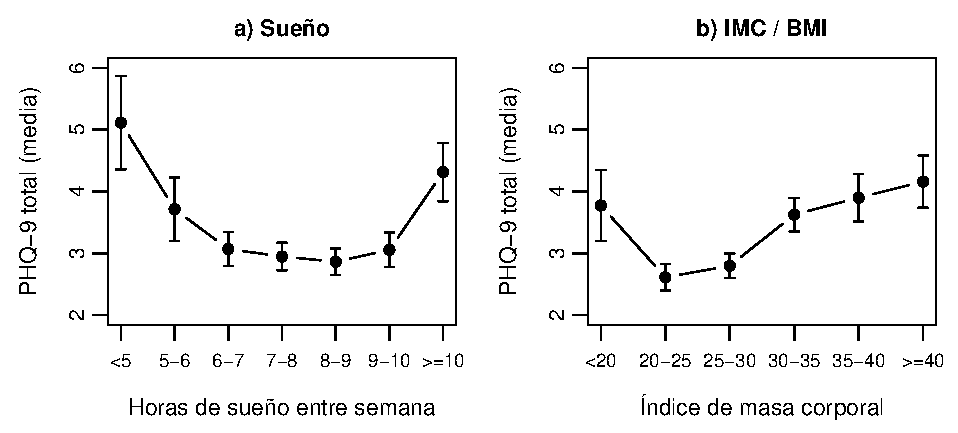
\includegraphics[width=\textwidth]{fig3_nhanes_es.pdf}
\figurenote{Medias y intervalos de confianza del 95 \% por categoría, adultos de NHANES 2017--2018 (sin pesos muestrales).}
\end{figure}

\begin{table}
\caption{Medidas de asociación entre la depresión (PHQ-9 total) y otras variables en NHANES}
\label{tab:s3nh}
\begin{threeparttable}
\small
\setlength{\tabcolsep}{4pt}
\begin{tabular}{lrcccc}
\toprule
Variable (frente a PHQ-9 total) & $n$ & Spearman $\rho$ ($p$) & $\xi_n$ ($p$) & dCor ($p$) & $\tau^*$ ($p$) \\
\midrule
Sue\~no entre semana (h) & 5032 & $-$.017 (.227) & .008 (.254) & .073 (.002)$^{\dagger}$ & .0009 ($<$ .001)$^{\dagger}$ \\
Sue\~no en fin de semana (h) & 5026 & $-$.029 (.042) & .011 (.357) & .074 (.002)$^{\dagger}$ & .0010 ($<$ .001)$^{\dagger}$ \\
\'Indice de masa corporal & 5010 & .102 ($<$ .001)$^{\dagger}$ & .012 (.268) & .117 (.002)$^{\dagger}$ & .0044 ($<$ .001)$^{\dagger}$ \\
Edad & 5068 & $-$.040 (.004)$^{\dagger}$ & .004 (.706) & .038 (.010)$^{\dagger}$ & .0008 ($<$ .001)$^{\dagger}$ \\
Raz\'on ingreso/pobreza & 4438 & $-$.170 ($<$ .001)$^{\dagger}$ & .024 (.017) & .177 (.002)$^{\dagger}$ & .0101 ($<$ .001)$^{\dagger}$ \\
G\'enero & 5068 & .138 ($<$ .001)$^{\dagger}$ & .019 (.180) & .123 (.002)$^{\dagger}$ & .0055 ($<$ .001)$^{\dagger}$ \\
\bottomrule
\end{tabular}

\begin{tablenotes}[flushleft]
\small
\item \textit{Nota.} Entre paréntesis, el valor $p$ (sin ajustar). Para $\xi_n$ se muestra el mayor de los dos sentidos y el $p$ combinado. $^{\dagger}$ Detecta la asociación según la regla ajustada por Benjamini--Hochberg. $p=.002$ es el menor valor alcanzable con 499 permutaciones.
\end{tablenotes}
\end{threeparttable}
\end{table}

\paragraph{Ruido por desempate.} Con ítems de pocas categorías, el valor de $\xi_n$ cambia con el desempate aleatorio tanto como su propio tamaño (Tabla~\ref{tab:s3tb}): la desviación estándar de $\xi_n$ entre desempates tuvo una mediana de .0139 en \texttt{bfi} y de .0120 en NHANES, frente a medianas de $|\xi_n|$ de .0167 y .0125. En el 40 \% de los pares de \texttt{bfi} y el 24 \% de los de NHANES la prueba de $\xi_n$ rechazó la independencia (con $\alpha=.05$) en entre el 25 \% y el 75 \% de los desempates, es decir, su decisión dependía del azar del desempate, al menos en un sentido.

\begin{table}
\caption{Variabilidad de $\xi_n$ entre desempates aleatorios en los datos reales}
\label{tab:s3tb}
\begin{threeparttable}
\small
\begin{tabular}{lcccc}
\toprule
 & Pares & DE de $\xi_n$ entre desempates (mediana) & $|\xi_n|$ (mediana) & Decisi\'on inestable (\%) \\
\midrule
\texttt{bfi} & 503 & .0139 & .0167 & 40 \\
NHANES & 127 & .0120 & .0125 & 24 \\
\texttt{sat.act} & 15 & .0264 & .0207 & 20 \\
\bottomrule
\end{tabular}

\begin{tablenotes}[flushleft]
\small
\item \textit{Nota.} Medianas entre pares del mayor de los dos sentidos. Decisión inestable: la prueba de $\xi_n$ cambió de decisión (con $\alpha=.05$) en entre el 25 \% y el 75 \% de los 20 desempates, en al menos un sentido.
\end{tablenotes}
\end{threeparttable}
\end{table}

\section{Discusión}

\subsection{Qué se encontró}

Los tres estudios dan una imagen coherente. Primero, la prueba de $\xi_n$ es válida en las condiciones habituales de los datos psicológicos --respuestas continuas, ordinales, puntajes compuestos y binarias balanceadas-- siempre que se use la versión con ajuste por empates; la versión que supone variables continuas rechaza el triple de lo debido con respuestas binarias. Se vuelve anticonservadora con respuestas binarias muy desbalanceadas (5 a 10 \% en una categoría), sobre todo en la cola, y el problema no desaparece con tamaños de muestra grandes. Segundo, $\xi_n$ es, con diferencia, la medida más potente ante relaciones oscilatorias, pero es mucho menos potente que las demás ante relaciones monótonas y, con efectos pequeños como los de la psicología, ante formas en U: dCor y $\tau^*$ son preferibles para éstas. Tercero, en los datos reales $\xi_n$ nunca detectó algo que Spearman y Pearson pasaran por alto; las asociaciones que éstos no vieron --como la forma de U entre sueño y depresión-- las detectaron dCor y $\tau^*$. Cuarto, con ítems de pocas categorías el valor de $\xi_n$ está dominado por el desempate aleatorio, y dicotomizar $X$ con una división por la mediana elimina la señal de las relaciones no monótonas simétricas, de modo que $\xi_n$ queda en el nivel nominal.

\subsection{Guía práctica}

La Tabla~\ref{tab:guia} resume qué medida usar según el tipo de relación que se sospecha. Además, se recomienda lo siguiente al reportar $\xi_n$: (a) usar la prueba con ajuste por empates (en \texttt{XICOR}, \texttt{ties = TRUE}, el valor por defecto) y no la que supone variables continuas; (b) indicar el sentido del coeficiente, $\xi_n(X,Y)$ o $\xi_n(Y,X)$; (c) cuando hay empates, promediar $\xi_n$ sobre varios desempates (aquí, 20) y reportar su desviación estándar, y no un único valor; (d) con una respuesta binaria cuya categoría minoritaria sea menor a alrededor del 5 \% (o a unos 50 casos), reportar el número de casos de esa categoría y preferir la prueba de permutación; (e) no reportar intervalos de confianza de $\xi_n$ obtenidos por bootstrap; y (f) no dicotomizar las variables continuas antes del análisis. Los puntajes compuestos no plantearon problemas.

\begin{table}
\caption{Guía para elegir una medida de asociación según la relación esperada}
\label{tab:guia}
\begin{threeparttable}
\small
\begin{tabular}{p{3.6cm}p{4.2cm}p{6.6cm}}
\toprule
Relación esperada & Medida recomendada & Advertencia \\
\midrule
Lineal o monótona & Pearson o Spearman & $\xi_n$ necesita unas ocho veces más participantes para la misma potencia ($R^2=.13$). \\
Forma de U o U invertida & dCor o $\tau^*$ (en este estudio, dCor fue la más potente); $\xi_n$ como complemento & Pearson y Spearman pueden valer cerca de cero (sueño y depresión: $\rho=-.017$). \\
Oscilatoria o funcional compleja & $\xi_n$ & Es la única que alcanza una potencia de .80 con $n\le 400$ ($n\approx 140$ con $R^2=.26$). \\
No funcional (por ejemplo, circular) & $\tau^*$; dCor con $n$ grande & $\xi_n$ es intermedia; ninguna medida detecta señales débiles ($R^2<.70$). \\
Exploración de muchos pares con efectos débiles & Spearman junto con dCor o $\tau^*$; graficar los pares detectados solo por las medidas generales & $\xi_n$ detectó menos pares que Spearman (138 frente a 434 en \texttt{bfi}). \\
\bottomrule
\end{tabular}
\begin{tablenotes}[flushleft]
\small
\item \textit{Nota.} Basada en los Estudios 1 a 3; las cifras corresponden a las condiciones simuladas.
\end{tablenotes}
\end{threeparttable}
\end{table}

\subsection{Limitaciones}

Las simulaciones usan variables latentes normales, cuatro estructuras de dependencia, una dependencia por vez y una sola variable explicativa; otras distribuciones o formas podrían cambiar los tamaños de muestra necesarios. La calibración por varianza explicada es una de varias escalas posibles, y la elegida no es útil para estructuras cuya señal reside en la varianza condicional. Las pruebas de permutación tienen resolución limitada (con 499 permutaciones el menor $p$ es .002), y los resultados de potencia con las cinco medidas se basan en 500 réplicas, de modo que las diferencias menores a unos .04 no deben interpretarse. En los datos reales, que dCor o $\tau^*$ detecten un par que Spearman no detecta no demuestra por sí solo una forma no monótona: con muestras de miles de personas incluso dependencias muy pequeñas resultan significativas, y la significación no equivale a relevancia práctica; en este trabajo solo se verificó gráficamente la forma de los pares de sueño e índice de masa corporal. El análisis de NHANES no usa pesos muestrales. Por último, $\xi_n$ se evaluó solo en su versión bivariada y sin intervalos de confianza, por las razones expuestas.

\subsection{Ciencia abierta}

Todo el código (generación de datos, pruebas, análisis, tablas y figuras) y los resultados crudos están disponibles en un repositorio público; las simulaciones y los análisis de datos reales se ejecutaron con flujos de trabajo de GitHub Actions con semillas fijas, y dos ejecuciones independientes de los bloques principales del Estudio 2 produjeron archivos idénticos byte a byte.

\section*{Declaraciones}

\paragraph{Financiamiento.} Este trabajo no recibió financiamiento específico.

\paragraph{Conflicto de intereses.} El autor declara no tener conflictos de intereses.

\paragraph{Aprobación ética y consentimiento.} No aplica: el estudio usa datos simulados y datos secundarios públicos sin información identificable.

\paragraph{Disponibilidad de datos y materiales.} Los datos \texttt{bfi} y \texttt{sat.act} están en el paquete \texttt{psych} de CRAN (\texttt{data(bfi, package = "psych")}; \texttt{data(sat.act, package = "psych")}). Los archivos de NHANES 2017--2018 (\texttt{DEMO\_J}, \texttt{DPQ\_J}, \texttt{SLQ\_J}, \texttt{BMX\_J}) se descargan sin registro de \url{https://wwwn.cdc.gov/Nchs/Data/Nhanes/Public/2017/DataFiles/}, y su tamaño y suma de verificación se registran en los resultados. Los resultados crudos de las simulaciones y de los análisis de datos reales están en \blindtext{\url{https://github.com/ArchieJamDev/ChatterjeeXi-Simulation}}{[enlace anónimo para la revisión]}.

\paragraph{Disponibilidad de código.} Todo el código está en el mismo repositorio (\blindtext{\url{https://github.com/ArchieJamDev/ChatterjeeXi-Simulation}}{[enlace anónimo para la revisión]}), con instrucciones de ejecución, semillas fijas y los flujos de trabajo de GitHub Actions con que se produjeron los resultados. Software: R \parencite{rcore2025}, \texttt{XICOR}, \texttt{energy}, \texttt{TauStar} y \texttt{psych}.

\paragraph{Contribución del autor.} Autor único: concepción, diseño, análisis, redacción.

\paragraph{Uso de herramientas de inteligencia artificial.} Se utilizó un asistente de inteligencia artificial (Claude, Anthropic) como apoyo para programar, ejecutar y verificar las simulaciones y los análisis, y para redactar borradores del texto. El autor revisó y verificó el código, los resultados y el texto, y es el único responsable del contenido.

\section*{Declaración de prácticas abiertas}

Los datos y el código de este estudio están disponibles públicamente (véase Disponibilidad de datos y materiales y Disponibilidad de código). Ninguna parte del estudio fue preinscrita; la regla de análisis del Estudio 3 (conjunto de pares, medidas y criterio de decisión) se fijó en el código antes de ejecutar los análisis, y el historial del repositorio lo documenta.

\printbibliography

\end{document}
